% The body of every paper in this folder: text, inline and display math, code, a table, a figure with a label in
% the sans-serif font, a footnote, and references.
\section{Introduction}
Flaky tests pass and fail on the same code without any change to the program under test. Such tests waste the
time of developers and hide real faults. This paper presents a detector that reruns each test in shuffled orders
and labels the test as \textit{stable}, \textit{flaky}, or \textit{unclear}. The detector runs as a plug-in of
\texttt{mvn test} and reads the reports of the Surefire plug-in.
\lipsum[1-2]

\section{Approach}
For a test $t$ and an order $o$, the detector records the outcome $r(t, o) \in \{\mathit{pass}, \mathit{fail}\}$.
A test is flaky when two orders give different outcomes, and the detector stops after $n$ orders with
\begin{equation}
\exists\, o_1, o_2 \colon r(t, o_1) \neq r(t, o_2), \qquad \sum_{i=1}^{n} \frac{x_i^2}{\sqrt{n}} \leq \alpha .
\end{equation}
\begin{lstlisting}[language=Java,basicstyle=\ttfamily\footnotesize]
@Test
public void testCache() {
    assertEquals(3, cache.size());
}
\end{lstlisting}
\lipsum[3-4]

\begin{table}[t]
\caption{Tests per label}
\centering
\begin{tabular}{lrr}
\toprule
Label & Tests & Percent \\
\midrule
stable & 450 & 84.4 \\
flaky & 51 & 9.6 \\
unclear & 32 & 6.0 \\
\bottomrule
\end{tabular}
\end{table}

\begin{figure}[t]
\centering
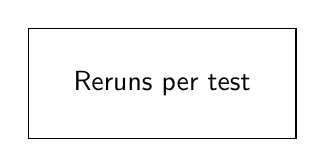
\begin{tikzpicture}
\draw (0,0) rectangle (3.4,1.4);
\node at (1.7,0.7) {\sffamily Reruns per test};
\end{tikzpicture}
\caption{The detector reruns each test in shuffled orders.}
\end{figure}

\section{Evaluation}
\lipsum[5-6]\footnote{The detector and its data are available to the reviewers.}

\section{Conclusion}
\lipsum[7]

\begin{thebibliography}{9}
\bibitem{a} A. Author and B. Author, ``A study of flaky tests,'' in \emph{Proc. Conf.}, 2020, pp. 1--10.
\bibitem{b} C. Author, ``Test order dependence in Java,'' \emph{J. Softw.}, vol. 3, no. 2, pp. 11--20, 2021.
\end{thebibliography}
